% Source PDF page 151 (printed p. 137)
\begin{itemize}
\item 目标函数必须是凸函数；
\item 不等式约束函数必须是凸函数；
\item 等式约束函数 $h_i(x)=a_i^\T x-b_i$ 必须是仿射函数。
\end{itemize}
由此立即得到一个重要性质：凸优化问题的可行集是凸集，因为它是问题定义域
\[
\mathcal D=\bigcap_{i=0}^m\dom f_i
\]
与 $m$ 个凸下水平集 $\{x\mid f_i(x)\le0\}$ 以及 $p$ 个超平面 $\{x\mid a_i^\T x=b_i\}$ 的交，而定义域本身也是凸集。（不失一般性，可假设 $a_i\ne0$：若某个 $i$ 满足 $a_i=0$、$b_i=0$，可删除第 $i$ 个等式约束；若 $a_i=0$、$b_i\ne0$，该等式约束不相容，问题不可行。）因此，在凸优化问题中，我们在凸集上最小化凸目标函数。

若 $f_0$ 是拟凸而非凸函数，就称问题（4.15）为标准形式拟凸优化问题。由于凸函数或拟凸函数的下水平集是凸集，可知凸优化或拟凸优化问题的 $\epsilon$ 次优集均为凸集。特别地，最优集是凸集。若目标严格凸，则最优集至多包含一个点。

\subsubsection*{凹函数最大化问题}
若 $f_0$ 凹，而不等式约束函数 $f_1,\ldots,f_m$ 凸，我们也稍微放宽用语，将
\begin{equation}
\begin{array}{ll}
\text{最大化}&f_0(x)\\
\text{约束为}&f_i(x)\le0,\quad i=1,\ldots,m,\\
&a_i^\T x=b_i,\quad i=1,\ldots,p
\end{array}\tag{4.16}
\end{equation}
称为凸优化问题。这个凹函数最大化问题可以通过最小化凸目标 $-f_0$ 容易地求解。我们针对最小化问题介绍的全部结果、结论和算法，都容易转到最大化情形。类似地，当 $f_0$ 为拟凹函数时，也称最大化问题（4.16）为拟凸问题。

\subsubsection*{抽象形式的凸优化问题}
凸优化问题的定义中有一点细微之处值得注意。考虑变量为 $x\in\R^2$ 的例子
\begin{equation}
\begin{array}{ll}
\text{最小化}&f_0(x)=x_1^2+x_2^2\\
\text{约束为}&f_1(x)=x_1/(1+x_2^2)\le0,\\
&h_1(x)=(x_1+x_2)^2=0.
\end{array}\tag{4.17}
\end{equation}
它具有标准形式（4.1）。此问题并不是标准形式凸优化问题，因为等式约束函数 $h_1$ 不是仿射函数，不等式约束函数 $f_1$ 也不是凸函数。

% Source PDF page 152 (printed p. 138)
但可行集 $\{x\mid x_1\le0,\ x_1+x_2=0\}$ 是凸集。因此，虽然此问题是在凸集上最小化凸函数 $f_0$，按照我们的定义，它仍不是凸优化问题。

当然，很容易把问题重新写为
\begin{equation}
\begin{array}{ll}
\text{最小化}&f_0(x)=x_1^2+x_2^2\\
\text{约束为}&\widetilde f_1(x)=x_1\le0,\\
&\widetilde h_1(x)=x_1+x_2=0,
\end{array}\tag{4.18}
\end{equation}
它具有标准凸优化形式，因为 $f_0$ 和 $\widetilde f_1$ 凸，而 $\widetilde h_1$ 仿射。

有些作者用“抽象凸优化问题”表示在凸集上最小化凸函数这一抽象问题。采用这种术语，问题（4.17）就是抽象凸优化问题。本书不采用这种术语。对我们而言，凸优化问题不仅是在凸集上最小化凸函数；还要求可行集由涉及凸函数的一组不等式和一组线性等式约束具体描述。问题（4.17）不是凸优化问题，而（4.18）是凸优化问题。（不过这两个问题是等价的。）

我们采用较严格的凸优化问题定义，在实践中影响不大。为求解在凸集上最小化凸函数的抽象问题，需要用凸不等式和线性等式约束描述该集合。如上例所示，这通常很直接。

\subsection{局部最优与全局最优}
凸优化问题的一项基本性质是：任何局部最优点也是全局最优点。为说明这一点，设 $x$ 为凸优化问题的局部最优点，即 $x$ 可行，且存在 $R>0$，使
\begin{equation}
f_0(x)=\inf\{f_0(z)\mid z\text{ 可行},\ \norm{z-x}_2\le R\}.\tag{4.19}
\end{equation}
假设 $x$ 不是全局最优点，即存在可行点 $y$ 满足 $f_0(y)<f_0(x)$。显然 $\norm{y-x}_2>R$，否则有 $f_0(x)\le f_0(y)$。考虑点
\[
z=(1-\theta)x+\theta y,\qquad\theta=\frac{R}{2\norm{y-x}_2}.
\]
此时 $\norm{z-x}_2=R/2<R$，且由可行集的凸性，$z$ 可行。又由 $f_0$ 的凸性，
\[
f_0(z)\le(1-\theta)f_0(x)+\theta f_0(y)<f_0(x),
\]
这与（4.19）矛盾。因此不存在满足 $f_0(y)<f_0(x)$ 的可行点 $y$，即 $x$ 全局最优。

% Source PDF page 153 (printed p. 139)
\begin{figure}[htbp]
\centering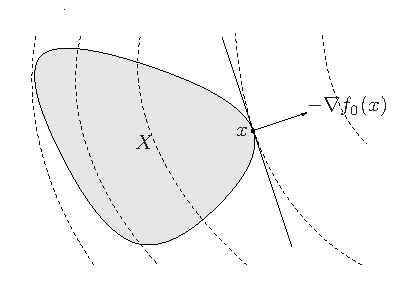
\includegraphics[width=.50\textwidth]{figures/ch04-02.pdf}
\caption*{图4.2\quad 最优性条件（4.21）的几何解释。阴影部分为可行集 $X$，虚线为 $f_0$ 的若干等高线。点 $x$ 最优：$-\nabla f_0(x)$ 在 $x$ 处定义了 $X$ 的一个支撑超平面（实线）。}
\end{figure}
拟凸优化问题的局部最优点不一定全局最优，见§4.2.5。

\subsection{可微目标函数 \texorpdfstring{$f_0$}{f0} 的最优性准则}
设凸优化问题的目标 $f_0$ 可微，因此对所有 $x,y\in\dom f_0$，有
\begin{equation}
f_0(y)\ge f_0(x)+\nabla f_0(x)^\T(y-x)\tag{4.20}
\end{equation}
（见§3.1.3）。用 $X$ 表示可行集，即
\[
X=\{x\mid f_i(x)\le0,\ i=1,\ldots,m,\ h_i(x)=0,\ i=1,\ldots,p\}.
\]
则 $x$ 最优，当且仅当 $x\in X$ 且
\begin{equation}
\nabla f_0(x)^\T(y-x)\ge0\qquad\text{对所有 }y\in X.\tag{4.21}
\end{equation}
这一最优性准则的几何意义是：若 $\nabla f_0(x)\ne0$，则 $-\nabla f_0(x)$ 在 $x$ 处定义可行集的一个支撑超平面，见图4.2。

\subsubsection*{最优性条件的证明}
先设 $x\in X$ 且满足（4.21）。对 $y\in X$，由（4.20）有 $f_0(y)\ge f_0(x)$。因此 $x$ 是问题（4.1）的最优点。

反过来，设 $x$ 最优，但条件（4.21）不成立，即存在 $y\in X$，使
\[
\nabla f_0(x)^\T(y-x)<0.
\]

% Source PDF page 154 (printed p. 140)
考虑点 $z(t)=ty+(1-t)x$，参数 $t\in[0,1]$。由于 $z(t)$ 位于 $x,y$ 之间的线段上，而可行集凸，所以 $z(t)$ 可行。我们断言，对充分小的正数 $t$，有 $f_0(z(t))<f_0(x)$，从而证明 $x$ 不最优。为此注意
\[
\left.\frac{d}{dt}f_0(z(t))\right|_{t=0}=\nabla f_0(x)^\T(y-x)<0,
\]
所以对充分小的正数 $t$，有 $f_0(z(t))<f_0(x)$。

第5章将更深入地研究最优性条件，这里先看几个简单例子。

\subsubsection*{无约束问题}
对于无约束问题，即 $m=p=0$，条件（4.21）化为熟知的最优性充要条件
\begin{equation}
\nabla f_0(x)=0.\tag{4.22}
\end{equation}
虽然我们已经见过这个最优性条件，仍有必要看看如何由（4.21）推出它。设 $x$ 最优，这里意味着 $x\in\dom f_0$，且对所有可行的 $y$ 有 $\nabla f_0(x)^\T(y-x)\ge0$。由于 $f_0$ 可微，其定义域按定义为开集，所以充分接近 $x$ 的所有 $y$ 都可行。取 $y=x-t\nabla f_0(x)$，其中 $t\in\R$ 为参数。$t$ 充分小且为正时，$y$ 可行，因此
\[
\nabla f_0(x)^\T(y-x)=-t\norm{\nabla f_0(x)}_2^2\ge0,
\]
从而 $\nabla f_0(x)=0$。

根据方程（4.22）解的个数，可能有几种情形。若（4.22）无解，就没有最优点，问题的最优值不能达到。这又可分为两种情形：问题无下界；或最优值有限但不能达到。另一方面，方程（4.22）也可能有多个解，此时每个解都是 $f_0$ 的最小点。

\begin{origexample}{4.5}
\textbf{无约束二次优化。}考虑最小化二次函数
\[
f_0(x)=(1/2)x^\T Px+q^\T x+r,
\]
其中 $P\in\mathbf S_+^n$，因此 $f_0$ 凸。$x$ 为 $f_0$ 最小点的充要条件是
\[
\nabla f_0(x)=Px+q=0.
\]
根据这个线性方程无解、有唯一解或有多个解，可能出现以下情形。
\begin{itemize}
\item 若 $q\notin\mathcal R(P)$，则无解。此时 $f_0$ 无下界。
\item 若 $P\succ0$（这也是 $f_0$ 严格凸的条件），则有唯一最小点 $x^\star=-P^{-1}q$。
% Source PDF page 155 (printed p. 141)
\item 若 $P$ 奇异，但 $q\in\mathcal R(P)$，则最优点构成仿射集 $X_{\mathrm{opt}}=-P^\dagger q+\mathcal N(P)$，其中 $P^\dagger$ 为 $P$ 的伪逆，见§A.5.4。
\end{itemize}
\end{origexample}

\begin{origexample}{4.6}
\textbf{解析中心。}考虑最小化凸函数 $f_0:\R^n\to\R$ 的无约束问题，其中
\[
f_0(x)=-\sum_{i=1}^m\log(b_i-a_i^\T x),\qquad\dom f_0=\{x\mid Ax\prec b\},
\]
$a_1^\T,\ldots,a_m^\T$ 为 $A$ 的各行。函数 $f_0$ 可微，所以 $x$ 最优的充要条件是
\begin{equation}
Ax\prec b,\qquad\nabla f_0(x)=\sum_{i=1}^m\frac{1}{b_i-a_i^\T x}a_i=0.\tag{4.23}
\end{equation}
（条件 $Ax\prec b$ 就是 $x\in\dom f_0$。）若 $Ax\prec b$ 不可行，则 $f_0$ 的定义域为空。假设 $Ax\prec b$ 可行，仍有以下几种可能，见习题4.2。
\begin{itemize}
\item （4.23）无解，因而问题没有最优点。当且仅当 $f_0$ 无下界时出现这种情形。
\item （4.23）有多个解。此时可以证明，解构成仿射集。
\item （4.23）有唯一解，即 $f_0$ 有唯一最小点。当且仅当开多面体 $\{x\mid Ax\prec b\}$ 非空且有界时出现这种情形。
\end{itemize}
\end{origexample}

\subsubsection*{只有等式约束的问题}
考虑有等式约束、没有不等式约束的情形，即
\[
\begin{array}{ll}\text{最小化}&f_0(x)\\\text{约束为}&Ax=b.\end{array}
\]
此时可行集是仿射集。假设它非空，否则问题不可行。对可行点 $x$，最优性条件要求
\[
\nabla f_0(x)^\T(y-x)\ge0
\]
对所有满足 $Ay=b$ 的 $y$ 成立。由于 $x$ 可行，每个可行点 $y$ 都可写为 $y=x+v$，其中 $v\in\mathcal N(A)$。所以最优性条件可以表示为
\[
\nabla f_0(x)^\T v\ge0\qquad\text{对所有 }v\in\mathcal N(A).
\]
一个线性函数若在子空间上非负，就必在该子空间上为零，所以对所有 $v\in\mathcal N(A)$ 有 $\nabla f_0(x)^\T v=0$。换言之，
\[
\nabla f_0(x)\perp\mathcal N(A).
\]

% Source PDF page 156 (printed p. 142)
利用 $\mathcal N(A)^\perp=\mathcal R(A^\T)$，最优性条件可写为 $\nabla f_0(x)\in\mathcal R(A^\T)$，即存在 $\nu\in\R^p$ 使
\[
\nabla f_0(x)+A^\T\nu=0.
\]
连同 $Ax=b$（即 $x$ 可行），这就是经典的拉格朗日乘子最优性条件，第5章将进一步研究。

\subsubsection*{非负正交象限上的最小化}
另一个例子是
\[
\begin{array}{ll}\text{最小化}&f_0(x)\\\text{约束为}&x\succeq0,\end{array}
\]
其中唯一的不等式约束是变量的非负约束。最优性条件（4.21）变为
\[
x\succeq0,\qquad\nabla f_0(x)^\T(y-x)\ge0\quad\text{对所有 }y\succeq0.
\]
除非 $\nabla f_0(x)\succeq0$，否则 $y$ 的线性函数 $\nabla f_0(x)^\T y$ 在 $y\succeq0$ 上无下界。于是条件化为 $-\nabla f_0(x)^\T x\ge0$。又由于 $x\succeq0$、$\nabla f_0(x)\succeq0$，必有 $\nabla f_0(x)^\T x=0$，即
\[
\sum_{i=1}^n(\nabla f_0(x))_ix_i=0.
\]
和式中每一项都是两个非负数的乘积，故每一项必为零，即 $(\nabla f_0(x))_ix_i=0$（$i=1,\ldots,n$）。所以最优性条件为
\[
x\succeq0,\qquad\nabla f_0(x)\succeq0,\qquad x_i(\nabla f_0(x))_i=0,\quad i=1,\ldots,n.
\]
最后一个条件称为互补性，因为它意味着向量 $x$ 和 $\nabla f_0(x)$ 的稀疏模式（非零分量对应的指标集合）互补，即交集为空。第5章还会遇到互补性条件。

\subsection{等价的凸问题}
了解§4.1.3中的哪些变换保持凸性是有用的。

\subsubsection*{消去等式约束}
凸问题的等式约束必须是线性的，即形如 $Ax=b$。此时，求一个特解 $x_0$ 和一个值域等于 $A$ 的零空间的矩阵 $F$，就可以消去等式约束，得到以 $z$ 为变量的问题

% Source PDF page 157 (printed p. 143)
\[
\begin{array}{ll}\text{最小化}&f_0(Fz+x_0)\\\text{约束为}&f_i(Fz+x_0)\le0,\quad i=1,\ldots,m.\end{array}
\]
由于凸函数与仿射函数复合仍凸，消去等式约束保持问题的凸性。此外，消去等式约束，以及由变换后问题的解恢复原问题的解，都只涉及标准线性代数运算。

至少在原则上，这意味着可以只考虑没有等式约束的凸优化问题。但许多情况下，保留等式约束更好，因为消去它们可能使问题更难理解和分析，或破坏求解算法的效率。例如，变量 $x$ 的维数很大，而消去等式约束会破坏问题的稀疏性或其他有用结构时，就会如此。

\subsubsection*{引入等式约束}
可以在凸优化问题中引入新变量和等式约束；只要这些等式约束是线性的，所得问题仍为凸问题。例如，若某个目标函数或约束函数形如 $f_i(A_ix+b_i)$，其中 $A_i\in\R^{k_i\times n}$，可引入新变量 $y_i\in\R^{k_i}$，用 $f_i(y_i)$ 替换 $f_i(A_ix+b_i)$，并加入线性等式约束 $y_i=A_ix+b_i$。

\subsubsection*{松弛变量}
引入松弛变量会产生新约束 $f_i(x)+s_i=0$。由于凸问题的等式约束函数必须是仿射函数，$f_i$ 必须仿射。换言之，为线性不等式引入松弛变量保持问题的凸性。

\subsubsection*{上图形式}
凸优化问题（4.15）的上图形式为
\[
\begin{array}{ll}
\text{最小化}&t\\
\text{约束为}&f_0(x)-t\le0,\\
&f_i(x)\le0,\quad i=1,\ldots,m,\\
&a_i^\T x=b_i,\quad i=1,\ldots,p.
\end{array}
\]
目标线性，因而凸；新约束函数 $f_0(x)-t$ 关于 $(x,t)$ 也凸，所以上图形式问题仍凸。

有时说线性目标对凸优化具有通用性，因为任何凸优化问题都容易变成具有线性目标的问题。凸问题的上图形式有若干实际用途。假定凸优化问题的目标线性，可以简化理论分析；也可以简化算法设计，因为求解线性目标凸优化问题的算法，借助上述变换，就能求解任意凸优化问题，只要它能够处理约束 $f_0(x)-t\le0$。

% Source PDF page 158 (printed p. 144)
\subsubsection*{对部分变量最小化}
对凸函数的部分变量最小化保持凸性。所以，若（4.9）中的 $f_0$ 关于 $x_1,x_2$ 联合凸，并且 $f_i$（$i=1,\ldots,m_1$）和 $\widetilde f_i$（$i=1,\ldots,m_2$）都凸，则等价问题（4.10）是凸问题。

\subsection{拟凸优化}
回顾标准形式的拟凸优化问题：
\begin{equation}
\begin{array}{ll}
\text{最小化}&f_0(x)\\
\text{约束为}&f_i(x)\le0,\quad i=1,\ldots,m,\\
&Ax=b,
\end{array}\tag{4.24}
\end{equation}
其中不等式约束函数 $f_1,\ldots,f_m$ 凸，目标 $f_0$ 拟凸，而凸优化问题要求目标凸。（拟凸约束函数可以用具有相同零下水平集的等价凸约束函数替换，见§3.4.5。）

本节指出凸优化与拟凸优化的一些基本区别，并说明如何将求解拟凸优化问题化为求解一系列凸优化问题。

\subsubsection*{局部最优解与最优性条件}
凸优化与拟凸优化最重要的区别是：拟凸优化问题可能存在并非全局最优的局部最优解。即使在 $\R$ 上无约束最小化拟凸函数的简单情形下，也能出现这一现象，如图4.3所示。

不过，§4.2.3中最优性条件（4.21）的一种变体，对目标可微的拟凸优化问题仍成立。以 $X$ 表示拟凸优化问题（4.24）的可行集。由拟凸性的一阶条件（3.20）可知，若
\begin{equation}
x\in X,\qquad\nabla f_0(x)^\T(y-x)>0\quad\text{对所有 }y\in X\setminus\{x\},\tag{4.25}
\end{equation}
则 $x$ 最优。与凸优化的对应准则（4.21）相比，有两个重要区别。
\begin{itemize}
\item 条件（4.25）只是最优性的充分条件；简单例子即可说明它对最优点未必成立。相比之下，（4.21）是 $x$ 解出凸问题的充要条件。
\item 条件（4.25）要求 $f_0$ 的梯度非零，而（4.21）没有这一要求。事实上，在凸情形下，$\nabla f_0(x)=0$ 时满足（4.21），$x$ 最优。
\end{itemize}

% Source PDF page 159 (printed p. 145)
\begin{figure}[htbp]
\centering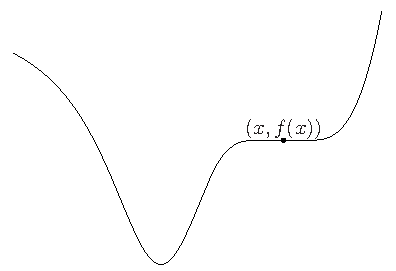
\includegraphics[width=.50\textwidth]{figures/ch04-03.pdf}
\caption*{图4.3\quad $\R$ 上的一个拟凸函数 $f$，其中局部最优点 $x$ 并非全局最优。这个例子说明，对凸函数有效的简单最优性条件 $f'(x)=0$，对拟凸函数并不成立。}
\end{figure}

\subsubsection*{通过凸可行性问题求解拟凸优化}
拟凸优化的一种一般方法，利用§3.4.5介绍的凸不等式族来表示拟凸函数的下水平集。设 $\phi_t:\R^n\to\R$（$t\in\R$）是一族凸函数，满足
\[
f_0(x)\le t\quad\Longleftrightarrow\quad\phi_t(x)\le0,
\]
而且对每个 $x$，$\phi_t(x)$ 关于 $t$ 非增，即 $s\ge t$ 时 $\phi_s(x)\le\phi_t(x)$。

以 $p^\star$ 表示拟凸优化问题（4.24）的最优值。如果可行性问题
\begin{equation}
\begin{array}{ll}
\text{求}&x\\
\text{使得}&\phi_t(x)\le0,\\
&f_i(x)\le0,\quad i=1,\ldots,m,\\
&Ax=b
\end{array}\tag{4.26}
\end{equation}
可行，则 $p^\star\le t$。反之，若（4.26）不可行，则 $p^\star\ge t$。问题（4.26）是凸可行性问题，因为全部不等式约束函数都凸，等式约束为线性。因此，可以通过求解凸可行性问题（4.26），判断拟凸优化问题的最优值 $p^\star$ 比给定值 $t$ 大还是小。若凸可行性问题可行，则 $p^\star\le t$，且任一可行点 $x$ 都对拟凸问题可行，并满足 $f_0(x)\le t$。若凸可行性问题不可行，则 $p^\star\ge t$。

这一观察可以构成一个简单的二分算法来求解拟凸优化问题（4.24），每一步解一个凸可行性问题。假设问题可行，先取一个已知包含最优值 $p^\star$ 的区间 $[l,u]$。在中点 $t=(l+u)/2$ 处求解凸可行性问题，判断最优值位于区间的下半段还是上半段，并据此更新区间。

% Source PDF page 160 (printed p. 146)
新区间仍包含最优值，但宽度只有原来的一半。重复这一过程，直到区间宽度足够小：

\begin{origalgorithm}{4.1}
\textbf{拟凸优化的二分法。}

给定 $l\le p^\star$、$u\ge p^\star$、容差 $\epsilon>0$。

重复：
\begin{enumerate}
\item $t:=(l+u)/2$。
\item 求解凸可行性问题（4.26）。
\item 若（4.26）可行，令 $u:=t$；否则令 $l:=t$。
\end{enumerate}
直到 $u-l\le\epsilon$。
\end{origalgorithm}

区间 $[l,u]$ 保证包含 $p^\star$，即每一步都有 $l\le p^\star\le u$。每轮将区间一分为二，因此 $k$ 轮后的区间长度为 $2^{-k}(u-l)$，这里 $u-l$ 指初始区间长度。由此可知，算法终止前恰需 $\lceil\log_2((u-l)/\epsilon)\rceil$ 轮。每一步都要求解凸可行性问题（4.26）。

\section{线性优化问题}
当目标函数和约束函数均为仿射函数时，问题称为线性规划（LP）。一般线性规划的形式为
\begin{equation}
\begin{array}{ll}
\text{最小化}&c^\T x+d\\
\text{约束为}&Gx\preceq h,\\
&Ax=b,
\end{array}\tag{4.27}
\end{equation}
其中 $G\in\R^{m\times n}$、$A\in\R^{p\times n}$。线性规划当然是凸优化问题。

由于目标中的常数 $d$ 不影响最优集或可行集，通常将它省略。仿射目标 $c^\T x+d$ 的最大化可以通过最小化 $-c^\T x-d$ 完成，后者仍凸，因此也把目标和约束函数均为仿射函数的最大化问题称为LP。

LP的几何意义如图4.4所示。LP（4.27）的可行集是多面体 $\mathcal P$；问题是在 $\mathcal P$ 上最小化仿射函数 $c^\T x+d$，或等价地最小化线性函数 $c^\T x$。

\subsubsection*{标准形式与不等式形式的线性规划}
LP（4.27）有两种非常常见的特殊情形，各有专门名称。标准形式LP中，唯一的不等式是逐分量非负约束 $x\succeq0$：
